\documentclass[10pt,a4paper]{article}
\usepackage[utf8]{inputenc}
\usepackage{amsmath}
\usepackage{amsfonts}
\usepackage{amssymb}

\usepackage{float}
\usepackage[table,xcdraw]{xcolor} %para usar tablas con color de fondo en las celdas
\usepackage{hyperref} %para poder poner enlaces
\usepackage{listings} %para insertar código
\usepackage{tikz}%para pintar las redes neuronales
\usepackage{color} %para poder definir y usar colores
\usepackage{soul} %para hacer los subrayados

\author{\textbf{Gustavo Rivas Gervilla}}
\title{\textcolor{deepblue}{\textbf{Redes Neuronales para MNIST}}}
\date{}

%Configurando lstlisting para mostrar código Python con algún esquema de colores (copiado de http://tex.stackexchange.com/questions/83882/how-to-highlight-python-syntax-in-latex-listings-lstinputlistings-command) ------------------------------
% Custom colors
\definecolor{deepblue}{rgb}{0,0,0.5}
\definecolor{deepred}{rgb}{0.6,0,0}
\definecolor{deepgreen}{rgb}{0,0.5,0}
\definecolor{light-gray}{gray}{0.85}
\definecolor{comment-gray}{gray}{0.65}
\definecolor{light-green}{rgb}{0.66,1,0.5}

% Default fixed font does not support bold face
\DeclareFixedFont{\ttb}{T1}{txtt}{bx}{n}{8} % for bold
\DeclareFixedFont{\ttm}{T1}{txtt}{m}{n}{8}  % for normal

%Configuración de los listings
\lstset{
	language=Python,
	basicstyle=\ttm,
	otherkeywords={self},             % Add keywords here
	keywordstyle=\ttb\color{deepblue},
	emph={MyClass,__init__},          % Custom highlighting
	emphstyle=\ttb\color{deepred},    % Custom highlighting style
	stringstyle=\color{deepgreen},
	frame=tb,                         % Any extra options here
	showstringspaces=false,            % 
	commentstyle=\ttm\color{comment-gray}, % Custom comment style
}
%--------------------------------------------------------------------------------

\newcommand{\code}[1]{\sethlcolor{light-gray}\hl{\texttt{#1}}} %Comando para poner código inline
\newcommand{\archive}[1]{\sethlcolor{light-green}\hl{\texttt{#1}}} %Comando para resaltar nombres de archivos
\renewcommand\tablename{Tabla} %Cambiar el nombre de las tablas
\renewcommand\figurename{Figura} %Cambiar el nombre de las tablas
\renewcommand{\contentsname}{Índice} %Cambiar el nombre de la ToC

\begin{document}
\maketitle
\begin{center}
\textbf{IC. Máster Universitario en Ingeniería Informática}
\newline
\newline
\newline

\includegraphics[scale=0.5]{img/decsai}
\end{center}

\newpage
\tableofcontents
\newpage

%Definición de variables para tikz
\def\layersep{2.5cm}

\section{Introducción}

En esta práctica se pretende probar distintos algoritmos de aprendizaje y topologías para redes neuronales a fin de identificar dígitos manuscritos en las imágenes de la base de datos MNIST. Se cuenta con 60000 muestras de entrenamiento y otras 10000 para testear la bondad de los algoritmos probados, que sería medida en términos de la tasa de error.\\

Las imágenes se cargarán de sendos ficheros comprimidos empleando el código que podemos encontrar en el fichero \archive{reader.py} el cuál se encarga de obtener cada imagen del fichero comprimido, formateando correctamente los bytes que se van leyendo de dicho fichero y normalizando las imágenes para su posterior almacenamiento (en el directorio \archive{data}) y uso. Para realizar esta descompresión y normalización nos hemos basado en el código Java facilitado por el profesor a tal efecto.

\section{Herramientas y entorno de desarrollo}
Para la realización de esta práctica hemos optado por emplear el lenguaje \textbf{Python 3} pese a que podemos pensar que no es tan eficiente como otros lenguajes, tiene la ventaja de contar con el módulo \textbf{Numpy} cuyas operaciones están programadas en código C lo que lo hace muy eficiente para realizar cálculos vectoriales.\\

No obstante nosotros vamos a trabajar con otro módulo Python llamado \href{http://deeplearning.net/software/theano/index.html}{Theano} el cuál nos permite, de un modo transparente, realizar cálculos en la GPU, lo que en la mayoría de los casos hará que los cálculos a realizar sean mucho más eficientes. Aunque hemos de tener cuidado ya que, en primer lugar los cálculos han de realizarse empleando float32 en lugar de float64 para que se puedan realizar efectivamente en la GPU (en caso de no poderse realizar en GPU automáticamente se lanzarán en CPU a no ser que empleemos el flag \textit{force\_devide=True}). Por otro lado habrá código que se ejecuten más lento en la GPU que en la CPU ya sea porque no los hemos programado bien o porque no suponen un volumen de trabajo suficiente como para que la sobrecarga de enviar la información a la GPU sea rentable.\\

A fin de poder emplear esta computación en GPU ejecutaremos el archivo \archive{reader.py} la instrucción \code{THEANO\_FLAGS=mode=FAST\_RUN,device=cpu,floatX=float32 python reader.py}.\\

En la \href{http://deeplearning.net/software/theano/tutorial/using_gpu.html}{página} de Theano donde se nos explica cómo usar la GPU hay un código de ejemplo el cuál se ejecuta en menos de 1/3 del tiempo que se consumiría ejecutando dicho código en CPU.

Por otro lado podemos encontrar un ejemplo sobre cómo programar una red neuronal que trabaje con minilotes de un modo eficiente usando la funcionalidad de Theano:

\begin{lstlisting}
import numpy as np

import theano
import theano.tensor as tensor

x = np.load('data_x.npy')
y = np.load('data_y.npy')

# symbol declarations
sx = tensor.matrix()
sy = tensor.matrix()
w = theano.shared(np.random.normal(avg=0, std=.1,
                                   size=(784, 500)))
b = theano.shared(np.zeros(500))
v = theano.shared(np.zeros((500, 10)))
c = theano.shared(np.zeros(10))

# symbolic expression-building
hid = tensor.tanh(tensor.dot(sx, w) + b)
out = tensor.tanh(tensor.dot(hid, v) + c)
err = 0.5 * tensor.sum(out - sy) ** 2
gw, gb, gv, gc = tensor.grad(err, [w, b, v, c])

# compile a fast training function
train = theano.function([sx, sy], err,
    updates={
        w: w - lr * gw,
        b: b - lr * gb,
        v: v - lr * gv,
        c: c - lr * gc})

# now do the computations
batchsize = 100
for i in xrange(1000):
    x_i = x[i * batchsize: (i + 1) * batchsize]
    y_i = y[i * batchsize: (i + 1) * batchsize]
    err_i = train(x_i, y_i)
\end{lstlisting}

Este código nos servirá de guía para implementar los distintos algoritmos sobre redes neuronales que probaremos en esta práctica. Destacaría dos cosas del código anterior: cómo se definen las funciones para ser compiladas a fin de trabajar en GPU y lo sencillo que resulta calcular el gradiente del error para realizar la propagación hacia atrás, por supuesto contamos con que dicha operación esté optimizada.\\

Las pruebas se realizarán en un ordeandor con \textbf{Arch Linux 64b}, \textbf{8 GB} de memoria RAM, un procesador \textbf{Intel Core i7-6700HQ} a 3.5 GHz y una tarjeta gráfica \textbf{NVIDIA GeForce GTX 950M}.

\section{Algoritmos basados en plantillas}

A continuación vamos a ver los primeros algoritmo de aprendizaje que vimos en clase y que son de un funcionamiento muy básico. Estos algoritmos podríamos decir que están basados en plantillas ya que tenemos una neurona por cada uno de los dígitos a distinguir y se irán actualizando los peso de cada una a fin de reforzar aquellos píxeles que forman parte del número que cada una ha de reconocer y se irán debilitando los pesos de los píxeles que no forman parte del dígito que tienen que reconer y que por tanto sólo puede llevar a la neurona, y por última instancia a la red, a confusión. Por esto decimos que estos algoritmos se basan en plantillas, cada neurona almacenará una plantilla 28x28 que le dará los pesos que necesita para reconocer el dígito concreto que ha de reconocer. Contemplearemos tres aproximaciones, con una topología que podríamos describir por medio del siguiente esquema:

\begin{center}
\begin{tikzpicture}[shorten >=1pt,->,draw=black!50, node distance=\layersep]
    \tikzstyle{every pin edge}=[<-,shorten <=1pt]
    \tikzstyle{entry}=[circle,fill=green!50,minimum size=5pt,inner sep=0pt]
    \tikzstyle{neuron}=[circle,fill=black!25,minimum size=10pt,inner sep=0pt]
    \tikzstyle{hidden neuron}=[neuron, fill=orange!50];
    \tikzstyle{annot} = [text width=4em, text centered]

    % Draw the input layer nodes
    \foreach \name / \y in {0,1}
    % This is the same as writing \foreach \name / \y in {1/1,2/2,3/3,4/4}
        \node[entry, pin=left:$pixel_{\y}$] (I-\name) at (0,-0.5*\y cm) {};
    
    \node at (-1,-0.5*3) {\vdots};
    \node[entry, pin=left:$pixel_{782}$] (I-782) at (0,-0.5*5) {};
    \node[entry, pin=left:$pixel_{783}$] (I-783) at (0,-0.5*6) {};

    % Draw the hidden layer nodes
    \foreach \name / \y in {0,...,9}
        \path[yshift=0.5cm]
            node[hidden neuron, pin={[pin edge={->}]right:$salida_{\y}$}] (H-\name) at (\layersep,-0.5*\y cm) {};

    % Connect every node in the input layer with every node in the
    % hidden layer.
    \foreach \source in {0,1,782,783}
        \foreach \dest in {0,...,9}
            \path (I-\source) edge (H-\dest);

    % Annotate the layers
    \node[annot,above of=H-0, node distance=1cm] (hl) {Salidas};
    \node[annot,left of=hl] {Entradas};    
\end{tikzpicture}
\end{center}

\subsection{Penalización fija por equivocación (Plantillas 1)}
\archive{algTemplates1.py}\\

Este algoritmo es muy sencillo, lo que hace es aumentar o disminuir una cantidad fija (\code{lr}) a aquellos pesos de la neurona que ha ganado la votación (que sería aquella tal que el valor $\underset{j = 0}{\overset{28^2-1}{\Sigma}} w_{ij}img_j$, donde $w_{ij}$ es el peso de la neurona i-ésima para el píxel $j$ de la imagen, es el más alto) correspondientes a los píxeles activos de la imagen; aquellos con un valor superior a cero en la imagen.\\

Hay que señalar que en caso de realizar esta actualización a todos los pesos de la neurona, en lugar de sólo a los activos, entonce el error sería mucho más grande (aprox. un 85\%). Esto se debe a que estamos trabajando con algoritmos que sólo cambian su información de aprendizaje según la imagen que le damos como entrada, entonces si aportamos información a través de pesos correspondientes a píxeles de la imagen que no contenían información, lo único que hacemos es ``confundir'' a la red.

\subsection{Penalización fija y refuerzo de neurona correcta (Plantillas 2)}
\archive{algTemplates2.py}\\

En este caso es mucho menor el tiempo al ejecutar el cógido en CPU que en GPU (en CPU tadamos menos de 3 segundos y en cambio en GPU tarda algo más de 25), es decir, tal y como está planteado el algoritmo la sobrecarga que supone trasladar la información a la GPU es mayor que el tiempo de ejecución del algoritmo en sí.\\

Hay algo que destacar y es que en una primera prueba se había omitido el vector de bias, y el error era ligeramente menor que al incorporarlo. En mi opinión esto se debe a que como estamos trabajando con un sistema de plantillas lo único que hacemos al incorporar este elemento es introducir una información que realmente es ficticia; la actualización de pesos viene sólo dada por los píxeles activos en la imagen de entrada.\\

Este algoritmo mejora sustancialmente al anterior en tasa de error puesto que no sólo se limita a penalizar o compensar a la neurona que dio la salida mayor, la que se consideraría para la clasificación, sino que además en todos los casos se refuerza aquella neurona que debería haber sido la que diese la clase correcta de la imagen.

\subsection{Actualización de pesos según el error (Plantillas 3)}
\archive{algTemplates3.py}\\

Para este algoritmo nos hemos basado en el siguiente enlace: \url{https://mmlind.github.io/Simple_1-Layer_Neural_Network_for_MNIST_Handwriting_Recognition/}. Lo primero que necesitaremos es algo que también vamos a necesitar cuando pasemos a trabajar con algoritmos de aprendizaje más sofisticados, pasamos de tener las etiquetas representadas por un número entero por tener cada una representada por un array binario que tiene un 1 sólamente en aquella posición correspondiente a la etiqueta. Este código también lo tenemos en el archivo \archive{reader.py} y almacena estas etiquetas en el archivo \archive{data/binTrainLbl.npy}.\\

Este algoritmo pretende contruir una plantilla pero empleando más información que la que usábamos en los dos algoritmo anteriores, ahora el incremento que se le añade a cada peso de la red neuronal es distinto en función del error cometido por la neurona a la que pertenece (diferencia entre el \textit{output} de esa neurona y la que debería ser, modelada por el vector binario anteriormente generado) y la entrada que se introdujo por esa dendríta de la neurona. Con lo cual el cambio que realizamos al peso viene dado según el error cometido y según el peso que tuviese el píxel de esa imagen en la salida de la neurona. Entonces si nos fijamos estamos ante un algoritmo que sólo actualiza los pesos relativos a píxeles activos en la imagen de entrada, como hacían los dos algoritmos anteriores, pero considerando más información que emplear una tasa de aprendizaje fija.

Tanto para este algoritmo como para los dos anteriores, dado que el tiempo de entrenamiento es muy reducido hemos optado por no almacenar los pesos de la red en un archivo para futuros usos, no obstante sí que fijamos la semilla aleatoria al inicio del algoritmo de modo que la inicialización de pesos de las neuronas sea siempre la misma. Se ha probado también a cambiar dicha semilla para asegurar que los resultados obtenidos no se deben al azar de los pesos obtenidos, y se han obtenido resultados muy similares.\\

Además la ejecución de este algoritmo nos ha permitido comprobar que lo que estamos haciendo en cuanto a la codificación de imágenes y las tasas de error calculadas es correcto, ya que obtenemos una tasa de error muy parecida a la que obtiene el desarrollador que ha publicado el algoritmo en el enlace anteriormente mencionado. Vamos ahora a mostrar el código desarrollado a fin de dar algunas ideas sobre la progración con \code{Theano}, que es lo que estamos empleado para las prácticas:\\

\begin{lstlisting}
import numpy as np
import time
import theano.tensor as T
from theano import function, config, scan, shared
from constants import *

np.random.seed(12345678)

lr = 0.1

imgs = np.load("data/trainImg.npy")
lbls = np.load("data/binTrainLbl.npy")
imgsTest = np.load("data/testImg.npy")
lblsTest = np.load("data/testLbl.npy")

x = T.vector('x')
y = T.vector('y')
A = T.matrix('A')

w = shared(np.random.rand(ROWS*COLS, 10).astype(config.floatX))

out = T.dot(x, w)/(28.0*28.0)
err = y - out
gw, aux = scan(lambda scalar,x: scalar * x, sequences=[err], non_sequences=x)

train = function([x, y], err, updates = {w: w + (lr * gw.T)})

#Train
t0 = time.time()
for img, lbl in zip(imgs, lbls):
    train(img, lbl)
t1 = time.time()

dot = function([x,A], T.dot(x,A))
#Test
predicted = []
nError = 0
for img, lbl in zip(imgsTest, lblsTest):
    p = np.argmax(dot(img, w.get_value()))
    predicted.append(p)
    if p != lbl:
        nError += 1
\end{lstlisting}

Lo primero que observamos es la fijación de la semilla aleatoria y la declaración de la tasa de aprendizaje, \code{lr}, a continuación cargamos todos los datos de la base. Ahora ya encontramos código de Theano, en primer lugar estamos definición unas variables simbólicas que nos servirán como base para definir otras tantas, con estas variables es con las que definimos las funciones Theano que serán compiladas.\\

Así denimos una variable \textit{shared}, \code{w}, que es una matriz $28^2 \mathrm{x} 10$ que representa los pesos de las diferentes neuronas que conforman la única capa de la topología que emplean estos algoritmos. La disponemos de este modo ya que después multiplicaremos un vector fila por ella y con lo cual las dimensiones tienen que ser las adecuadas.\\

A continuación definimos la variable que representará la salida, como vemos esta variable será el resultado de multiplicar el vector, que será la variable de entrada, por cada columna de la matriz, normalizado de modo que la salida quede en el [0,1]. Y definimos el error como un vector que será la diferencia entre el vector esperado, que representa la clase de la imagen de entrada, y la salida obtenida.\\

Ahora vamos a calcular la matriz de incrementos para la matriz de pesos, \code{gw}, esto lo hacemos por medio de la función \code{scan} de Theano que es algo parecido a los bucles de Theano que resultan algo más rápidos que un for usual; se realizó un pequeó experimento y se notó la diferencia de tiempos. Con esto definimos una nueva variable que almacena el resultado de multiplicar la entrada (representada por la variable simbólica \code{x}) por el error de cada una de las neuronas, representado por el vector simbólico \code{err}, que se recorre elemento a elemento y por esto se añada a la lista de \code{sequences} de la función \code{scan}; con la variable aux sólo recogemos el otro elemento devuelto por esta función que no vamos pasar a explicar pues no nos interesa en este momento.\\

Por último definimos una función Theano con el comando \code{function} que recibe como entradas dos vectores, que serán la imagen y el vector binario que codifica la clase, que calcula la variable \code{err} para dichas entradas y actualiza la matriz de pesos, \code{w}, sumándole la matriz de incrementos que se deriva del error multiplicada por la tasa de aprendizaje.\\

Después recorremos en un bucle usual de Python las imágenes de entrenamiento junto con sus vectores binarios de etiquetas y usamos la función que acabamos de definir para ir actualizando los pesos de la matriz según la salida obtenida para estas imágenes. Luego no hacemos más que emplear la red entrenada para obtener la clase que nos da para las imágenes de test, que será la correspondiente a la salida más alta de las diez neuronas (por esto empleamos \code{argmax}) y calculamos el número de errores obtenido. Observemos que también hemos definido una función para calcular el producto de un vector por una matriz con tal propósito.

\section{Backpropagation}

A continuación vamos a pasar a trabajar con neuronas que emplean el \newline mecanismo de propagación hacia atrás para actualizar los pesos de las neuronas que la forman, empezaremos con una red simple con una sola capa oculta y después iremos aumentando la complejidad de la topología de red empleada. Así la topología que tendremos de inicio será la siguiente será la siguiente:

\begin{center}
\begin{tikzpicture}[shorten >=1pt,->,draw=black!10, node distance=\layersep]
    \tikzstyle{every pin edge}=[<-,shorten <=1pt]
    \tikzstyle{neuron}=[circle,fill=black!25,minimum size=10pt,inner sep=0pt]
    \tikzstyle{input neuron}=[neuron, fill=green!50, minimum size=5pt];
    \tikzstyle{output neuron}=[neuron, fill=orange!50, minimum size =10pt];
    \tikzstyle{hidden neuron}=[neuron, fill=gray!50];
    \tikzstyle{annot} = [text width=4em, text centered]

    % Draw the input layer nodes
    \foreach \name / \y in {0,1}
    % This is the same as writing \foreach \name / \y in {1/1,2/2,3/3,4/4}
        \node[input neuron, pin=left:$pixel_{\y}$] (I-\name) at (0,-0.5*\y cm) {};
    
    \node at (0,-0.5*3) {\vdots};
    \node[input neuron, pin=left:$pixel_{782}$] (I-782) at (0,-0.5*5) {};
    \node[input neuron, pin=left:$pixel_{783}$] (I-783) at (0,-0.5*6) {};

    % Draw the hidden layer nodes
    \node at (\layersep,-0.5*3) {\vdots};
    \foreach \name / \y in {0,1,7,8}
        \path[yshift=0.5cm]
            node[hidden neuron] (H-\name) at (\layersep,-0.5*\y cm) {};
    
    %Draw output layer nodes  
    \foreach \name / \y in {0,...,9}
        \path[yshift=0.5cm]
            node[output neuron, pin={[pin edge={->}]right:$salida_{\y}$}] (O-\name) at (2*\layersep,-\y*0.5 cm) {};

    % Connect every node in the input layer with every node in the
    % hidden layer.
    \foreach \source in {0,1,782,783}
        \foreach \dest in {0,1,7,8}
            \path (I-\source) edge (H-\dest);

    % Connect every node in the hidden layer with the output layer
    \foreach \source in {0,1,7,8}
    		\foreach \dest in {0,...,9}
        		\path (H-\source) edge (O-\dest);

    % Annotate the layers
    \node[annot,above of=H-0, node distance=1cm] (hl) {Capa oculta};
    \node[annot,left of=hl] {Entradas};
    \node[annot,right of=hl] {Salidas};
\end{tikzpicture}
\end{center}

Los experimentos realizados para ajustar los parámetros de la red se han realizado atendiendo a la tasa de error en el conjunto de test. En la práctica deberían hacerse sobre un conjunto de validación, pero para poder emplear todas las muestras de entrenamiento disponibles para entrenar la red hemos optado por esta opción.\\

Gracias a la posibilidad de realizar cálculo simbólico con la libería Theano implementar los algoritmos de este estilo resulta muy sencillo ya que no necesitamos calcular el gradiesnte del error respecto a los distintos pesos de la red neuronal para poder propagar el error. Simplemente tenemos que realizar una declaración de variables simbólicas como la que se muestra en el siguiente framento de código que extraído del archivo \archive{backSoft.py}.

\begin{lstlisting}
W1 = shared(np.random.normal(loc=0, scale=.1, size=(784, nHidden))
.astype(config.floatX), name = 'W1')
b1 = shared(np.random.normal(loc=0, scale=.1, size=nHidden)
.astype(config.floatX), name = 'b1')
W2 = shared(np.random.normal(loc=0, scale=.1, size=(nHidden, 10))
.astype(config.floatX), name = 'W2')
b2 = shared(np.random.normal(loc=0, scale=.1, size=10)
.astype(config.floatX), name = 'b2')


hid = 1.0 / (1.0 + T.exp(-(T.dot(x, W1) + b1)))
out = 1.0 / (1.0 + T.exp(-(T.dot(hid, W2) + b2)))
y_hat = T.nnet.softmax(out)
err = - T.sum(y * T.log(y_hat))
prediction = T.argmax(y_hat)

#define gradients
dW1, db1, dW2, db2 = T.grad(err, [W1, b1, W2, b2])
\end{lstlisting}

Como podemos ver declaramos diversas variables simbólicas entre las que se encuentran las matrices de pesos de la red, y definimos una variable simbólica \code{err} que representa el error de entropía cruzada, que es la función de coste asociada a una capa de salida de tipo softmax. Finalmente definimos las variables \code{dW1, db1, dW2, db2}, que serán las derivadas de dicho error con respecto a las distintas matrices y vectores de pesos de la red haciendo uso de la función \code{grad} de la biblioteca Theano.

\subsection{Softmax}
\archive{backSoft.py}\\

Siguiendo los experimentos de los que se hablan en el guión de la práctica hemos implementado el algoritmo de backpropagation haciendo uso de una capa de salida de tipo softmax.\\

Para implementar esta capa de salida hemos hecho uso, como se muestra en el código que hemos mostrado anteriormente, de la función \code{softmax} de Theano. Y hemos de definir el error como el error de entropía cruzada, ya que si por ejemplo definimos el error como el error cuadrático medio, la tasa de error aumentará mucho. Además pese a que Theano dispone de una función para calcular este error, nos daba un error en cuanto al tipo del vector de salidas, con lo cual simplemente hemos definimo nosotros mismos tal error, que como vemos resulta muy cómodo: el opuesto de la sumatoria del producto de cada salida de la red con la salida esperada; hacemos uso de la clase de cada imagen representada por medio de un vector binario. Los experimentos que hemos realizado sobre este algoritmo se han centrado en modificar el número de neuronas de la capa oculta así como la tasa de aprendizaje a fin de poder ver sus efectos.\\

Comenzamos el experimento con una capa oculta con 256 neuronas al igual que en el ejemplo planteado en el guión de la práctica. En un principio empleamos la tangente hiperbólica como función de activación, esto simplemente implica cambiar la declaración de las variables simbólicas que representan la salida de las dos capas de la red:

\begin{lstlisting}
#tanh like activation function
# hid = T.tanh(T.dot(x, W1) + b1)
# out = T.tanh(T.dot(hid, W2) + b2)

#sigmoid like activation function
hid = 1.0 / (1.0 + T.exp(-(T.dot(x, W1) + b1)))
out = 1.0 / (1.0 + T.exp(-(T.dot(hid, W2) + b2)))

#Lecun recommended tanh like activation function
# hid = 1.7159 * T.tanh(0.67 * (T.dot(x, W1) + b1) )
# out = 1.7159 * T.tanh(0.67 * (T.dot(hid, W2) + b2) )
\end{lstlisting}

El emplear esta función de activación hace que la tasa de error (9.68\%) sea algo mayor que la obtenida empleando la función logística, con lo cual, al igual que en el experimento del que estamos partiendo, emplearemos la función logística como función de activación para las neuronas de la red. Una vez fijada la función de activación y la de coste hemos pasado a experimentar con el número de neuronas en la capa oculta así como el número de pasadas que realizamos sobre el conjunto de entrenamiento. También se probó con la tangente hiperbólica con los coeficientes $a$ y $b$ propuestos por Yann Lecun pero también obteníamos un error mayor que el obtenido con la función logística con lo que optamos por ésta.\\

\begin{figure}[H]
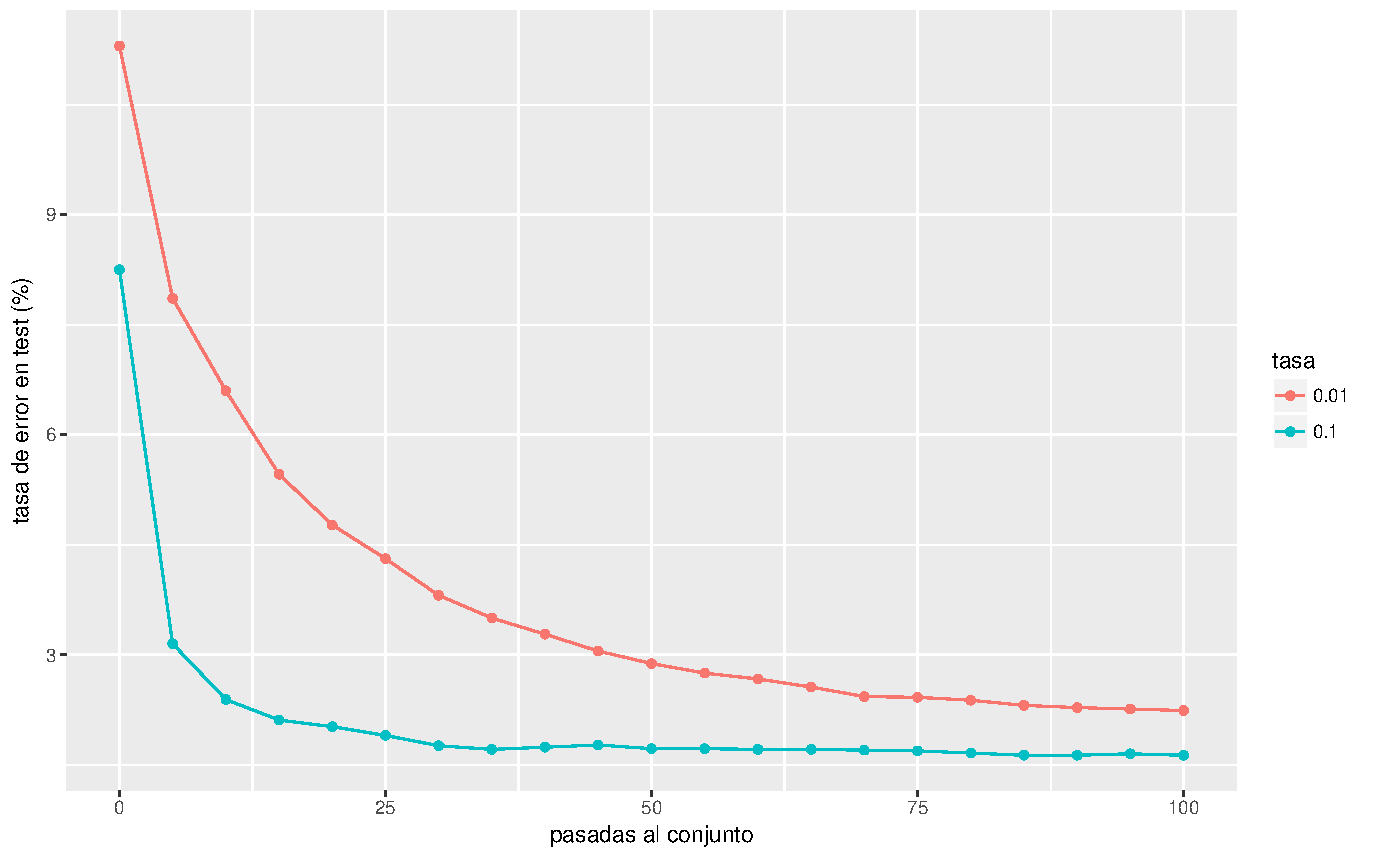
\includegraphics[scale=0.5]{img/tasa.pdf}
\caption{Comparación de tasas de apredizaje}
\end{figure}

\subsection{Momentos}
\archive{backSoftMomentums.py}

\begin{center}
\begin{table}[H]
\centering
\caption{Experimentos backpropagation}
\label{my-label}
\begin{tabular}{|c|c|c|c|c|c|}
\hline
\rowcolor[HTML]{FFFC9E} 
\textbf{\begin{tabular}[c]{@{}c@{}}Función\\ activación\end{tabular}} & \textbf{Error}   & \textbf{\begin{tabular}[c]{@{}c@{}}Nº neuronas\\ ocultas\end{tabular}} & \textbf{\begin{tabular}[c]{@{}c@{}}Tiempo\\ entrenamiento\\ (s)\end{tabular}} & \textbf{\begin{tabular}[c]{@{}c@{}}Tasa\\ error\\ (\%)\end{tabular}} & \textbf{\begin{tabular}[c]{@{}c@{}}Pasadas\\ al cojunto de \\ entrenamiento\end{tabular}} \\ \hline
tanh                                                                  & entropía cruzada & 256                                                                    & 14.52                                                                         & 9.68                                                                 & 1                                                                                         \\ \hline
logística                                                             & entropía cruzada & 256                                                                    & 12.53                                                                         & 7.57                                                                 & 1                                                                                         \\ \hline
logística                                                             & cuadrático medio & 256                                                                    & 12.75                                                                         & 90.68                                                                & 1                                                                                         \\ \hline
logística                                                             & entropía cruzada & 700                                                                    & 33.87                                                                         & 8.25                                                                 & 1                                                                                         \\ \hline
logística                                                             & entropía cruzada & 256                                                                    & 250.19                                                                        & 2.17                                                                 & 20                                                                                        \\ \hline
logística                                                             & entropía cruzada & 256                                                                    & 570.24                                                                        & 1.91                                                                 & 50                                                                                        \\ \hline
\end{tabular}
\end{table}
\end{center}







\begin{center}
\begin{tikzpicture}[shorten >=1pt,->,draw=black!50, node distance=\layersep]
    \tikzstyle{every pin edge}=[<-,shorten <=1pt]
    \tikzstyle{neuron}=[circle,fill=black!25,minimum size=17pt,inner sep=0pt]
    \tikzstyle{input neuron}=[neuron, fill=green!50];
    \tikzstyle{output neuron}=[neuron, fill=red!50];
    \tikzstyle{hidden neuron}=[neuron, fill=blue!50];
    \tikzstyle{annot} = [text width=4em, text centered]

    % Draw the input layer nodes
    \foreach \name / \y in {1,...,4}
    % This is the same as writing \foreach \name / \y in {1/1,2/2,3/3,4/4}
        \node[input neuron, pin=left:Input \#\y] (I-\name) at (0,-\y) {};

    % Draw the hidden layer nodes
    \foreach \name / \y in {1,...,5}
        \path[yshift=0.5cm]
            node[hidden neuron] (H-\name) at (\layersep,-\y cm) {};

    % Draw the output layer node
    \node[output neuron,pin={[pin edge={->}]right:Output}, right of=H-3] (O) {};

    % Connect every node in the input layer with every node in the
    % hidden layer.
    \foreach \source in {1,...,4}
        \foreach \dest in {1,...,5}
            \path (I-\source) edge (H-\dest);

    % Connect every node in the hidden layer with the output layer
    \foreach \source in {1,...,5}
        \path (H-\source) edge (O);

    % Annotate the layers
    \node[annot,above of=H-1, node distance=1cm] (hl) {Capa oculta};
    \node[annot,left of=hl] {Entradas};
    \node[annot,right of=hl] {Salida};
\end{tikzpicture}
\end{center}

\section{Resumen de resultados}

\begin{table}[H]
\centering
\caption{Resumen de resultados}
\label{my-label}
\begin{tabular}{|
>{\columncolor[HTML]{FFFFC7}}c |c|c|c|c|c|}
\hline
\cellcolor[HTML]{FFFC9E}\textbf{Algoritmo} & \cellcolor[HTML]{9AFF99}\textbf{\begin{tabular}[c]{@{}c@{}}Archivo\\ algoritmo\end{tabular}} & \cellcolor[HTML]{9AFF99}\textbf{\begin{tabular}[c]{@{}c@{}}Archivo \\ pesos\end{tabular}} & \cellcolor[HTML]{FD6864}\textbf{\begin{tabular}[c]{@{}c@{}}\% Error\\ entrenamiento\end{tabular}} & \cellcolor[HTML]{FD6864}\textbf{\begin{tabular}[c]{@{}c@{}}\% Error\\ test\end{tabular}} & \cellcolor[HTML]{FFFFFF}\textbf{\begin{tabular}[c]{@{}c@{}}Tiempo \\ entrenamiento\end{tabular}} \\ \hline
Plantillas 1                               & algTemplates1.py                                                                             & -                                                                                         &                                                                                                   &                                                                                          &                                                                                                  \\ \hline
Plantillas 2                               & algTemplates2.py                                                                             & -                                                                                         &                                                                                                   &                                                                                          &                                                                                                  \\ \hline
Plantillas 3                               & algTemplates3.py                                                                             & -                                                                                         &                                                                                                   &                                                                                          &                                                                                                  \\ \hline
Back +softmax                               & backSoft.py                                                                             & -                                                                                         &                                                                                                   &                                                                                          &                                                                                                  \\ \hline
\end{tabular}
\end{table}

\section{Manual de usuario}

\section{Bibliografía}

\begin{itemize}
	\item \href{http://deeplearning.net/software/theano/index.html}{Documentación Theano}
	\item \href{http://www.wildml.com/2015/09/speeding-up-your-neural-network-with-theano-and-the-gpu/}{Usando Theano para implementar backpropagation}
	\item \url{http://deeplearning.net/tutorial/mlp.html} (no usado)
\end{itemize}


\end{document}